\documentclass[a4paper,12pt]{article}
\usepackage{graphicx}
\author{Didrik Jonassen, Imre Kerr\vspace{-2ex}}
\title{\vspace{-12ex}Project 2\\ IT3708 --- Subsymbolic methods in AI}
\date{\today}

\begin{document}

\maketitle

\section{Description of Code}

\paragraph{}To begin with, we decided to do a major rewrite of the base EA system, based on things we had learned in the previous assignment. The system design is now much more modular and consistent. For instance, every functional unit used in the loop is now a function that accepts a population and returns a population, and they are all used in the same way (by passing them as parameters to the main loop).

\subsection{Overview}
\paragraph{}The entry point of the program is the problem-specific script \texttt{izzy.py}. It generates all the functions needed by the main EA loop by calling \textit{generator functions}, which prompt the user for parameters such as selection mechanisms, mutation rates etc. Some of the functions can be used as is, without decoration. It then gets a few more parameters (population size, max generations, fitness goal), generates the initial population, and passes all of this to the main EA loop (in \texttt{ea/main.py}). This loop runs until max generations or the fitness goal has been reached, and returns a list of the population for every generation. This list is passed to the \texttt{visualize} function, which plots the best spiketrain and the fitness graph using matplotlib. The parameter values and fitness of the best solution are printed to standard output.

\subsection{Genotype Representation}

\paragraph{}Rather than using a bit-vector for the genotype, we opted to use a list of float values directly, one for each parameter value. This allowed us to use fancier mutation and crossover functions:
\begin{itemize}
\item{\textbf{Gaussian difference mutation} --- Adds a gaussian random value to each float with a given probability. The standard deviation of this value is given as a fraction of the range of each variable.}
\item{\textbf{Uniform value mutation} --- Sets each value to a uniformly distributed new value with a given probability.}
\item{\textbf{Random choice crossover} --- Crosses two genomes by randomly choosing values from one or the other.}
\item{\textbf{Randomly weighted average crossover} --- For each parameter $p$ with parent values $p_a$ and $p_b$, generates a random value $x \in [ 0, 1 \rangle$, and sets $p = x p_a + (1-x)p_b$.}
\end{itemize}

\subsection{Fitness and Development}

\paragraph{}Since we already have distance metrics, our fitness function is simply $\frac{1}{1+dist}$. This has the nice property of maximum fitness always being $1.0$. The distance and development functions are basically given in the assignment text, so no further description of these is necessary. However, we did find that these were quite computationally intensive, and there was a lot of speedup to be had by adding multiprocessing support for these functions.

\section{Test Cases}

\paragraph{}For all of these, the EA parameters are as follows unless otherwise noted: \\

\begin{tabular}{ll}
\hline
Parameter & Value \\
\hline \hline
Population size & 100 \\
Adult selection & Generational mixing \\
Litter size & 100 \\
Parent selection & Sigma scaling \\
Mutation type & Gaussian \\
Mutation rate & 0.4 \\
Mutation std.dev. & 0.2 \\
Crossover type & Random choice \\
Max generations & 500 \\
Fitness goal & 1.0 \\
\hline
\end{tabular}
\subsection{Training Data Set 1}
\subsubsection{Waveform Distance Metric}
\centerline{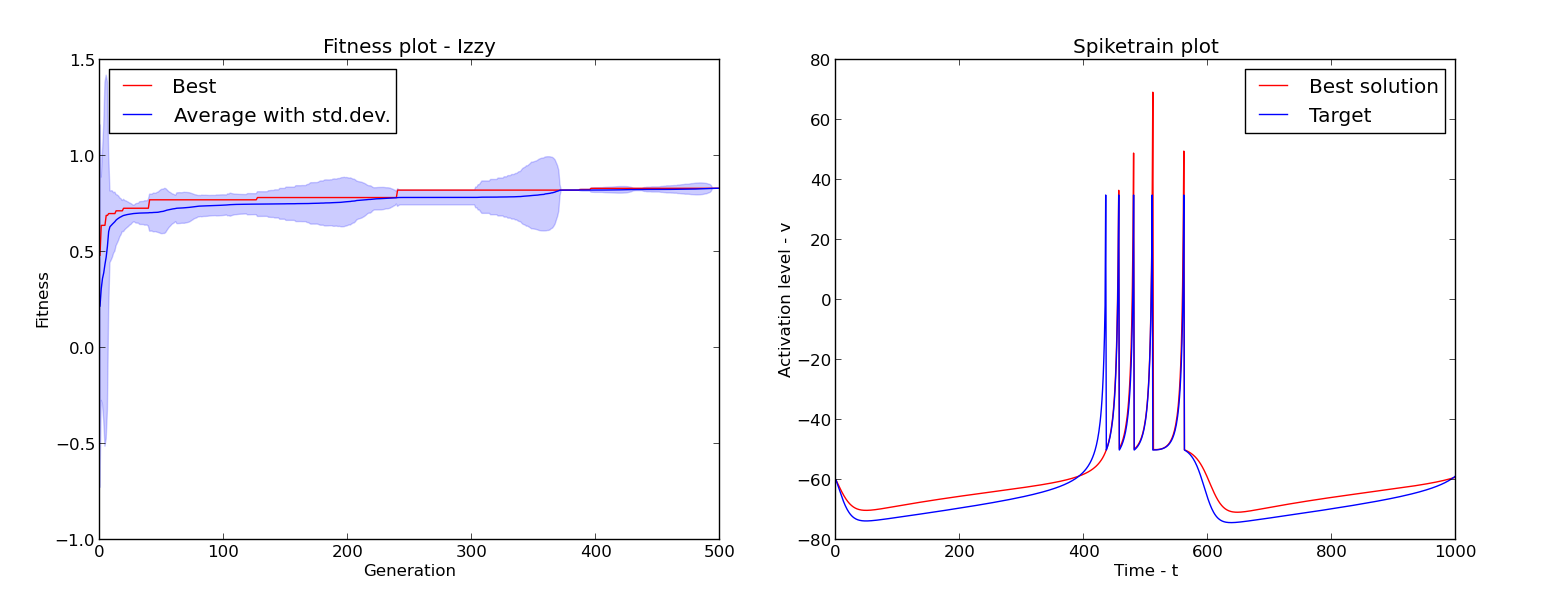
\includegraphics[width=1.2\textwidth]{img/case1_wave}}
% [0.07191327279747756, 0.08117384128793065, -49.85092625396891, 2.1621887697736297, 0.04047259008452674]
% 0.831769696586
Best solution: 
a: 0.07191 
b: 0.08117 
c: -49.85 
d: 2.162 
k: 0.04047 \\
Fitness: 0.8317
\paragraph{}The waveform distance metric gives a pretty good result, but looking closely we see that the first spike is actually missing. This highlights a problem with the waveform metric. Since spikes are so narrow, a spike or two can be missing without too much penalty.

\subsubsection{Spike Time Distance Metric}
\centerline{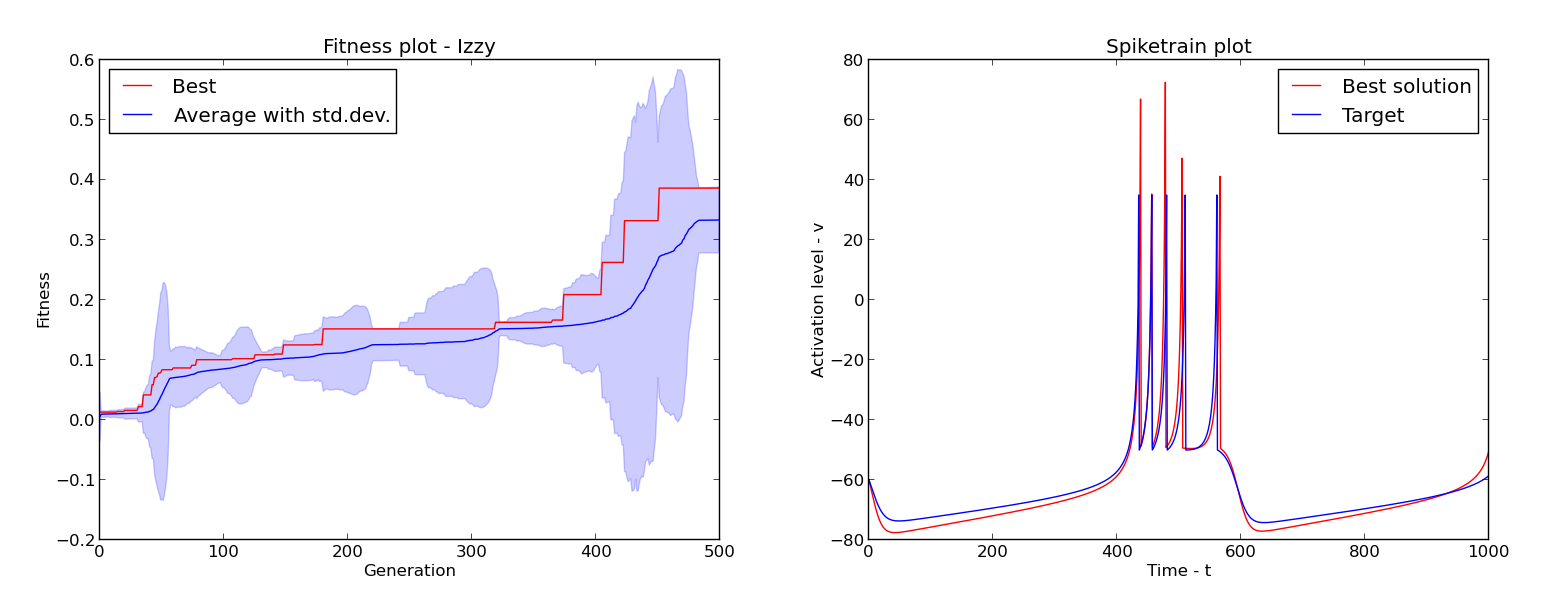
\includegraphics[width=1.2\textwidth]{img/case1_time}}
% [0.024175302012112966, 0.2438159164449954, -49.33954348796303, 2.506245585268969, 0.039253473712978035]
% 0.386480780683
Best solution: 
a: 0.02418 
b: 0.2438 
c: -49.34 
d: 2.506 
k: 0.0393 \\
Fitness: 0.3865
\paragraph{}The spike time metric yields a very good result in this case. We had to up the mutation standard deviation to 0.5, otherwise we'd end up with some very odd spiketrains as the algorithm would stagnate at some poor local maximum. We think this is because spiketrains similar to the target occupy a very small part of the solution space, so you have to explore a bit to get something that's close enough to work from. Also note the fact that the fitness increases over the entire run, so there's probably some room for improvement if we let it run longer.

\subsubsection{Spike Interval Distance Metric}
\centerline{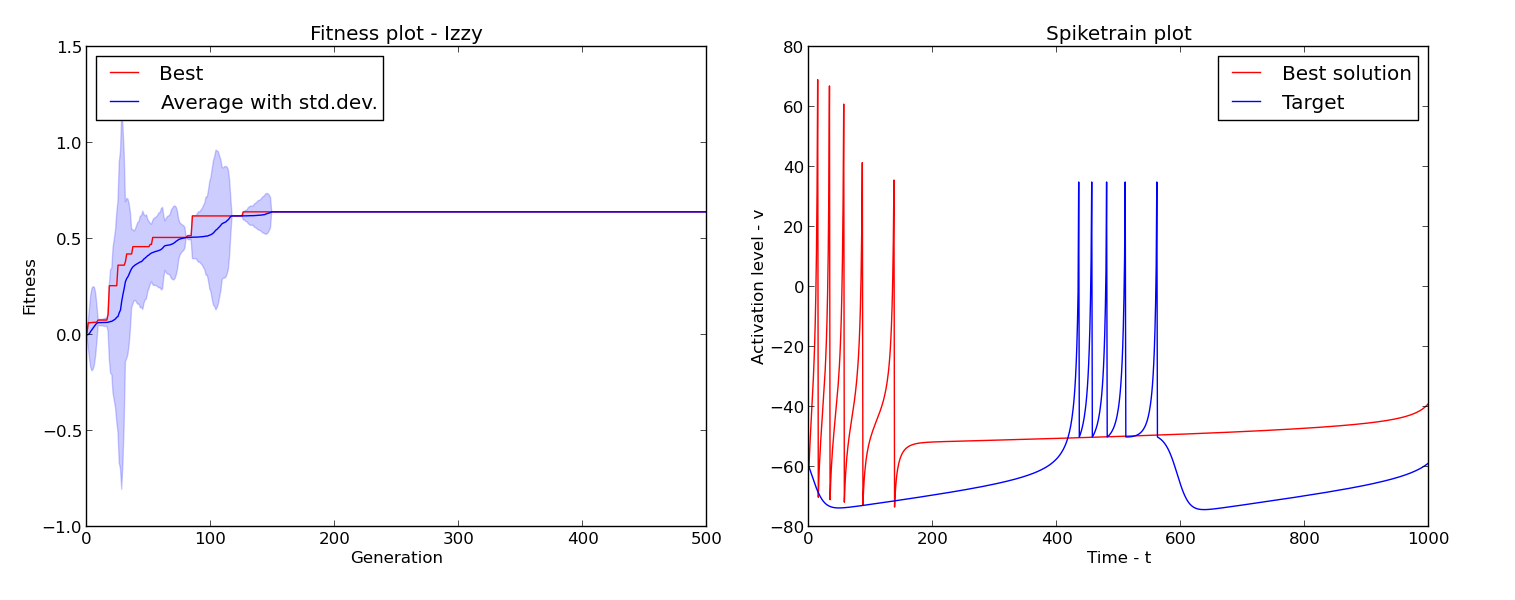
\includegraphics[width=1.2\textwidth]{img/case1_int}}
% [0.001, 0.01, -80.0, 8.244754856968658, 0.055851099927500036]
% 0.641429826364
Best solution: 
a: 0.001 
b: 0.01 
c: -80 
d: 8.2448 
k: 0.0559 \\
Fitness: 0.6414
\paragraph{}Here we see one weakness of the spike interval method. It pays no attention to the position of the spikes, only the intervals between them. In this case, we therefore end up with a radically different spiketrain.

\subsection{Training Data Set 2}
\subsubsection{Waveform Distance Metric}
\centerline{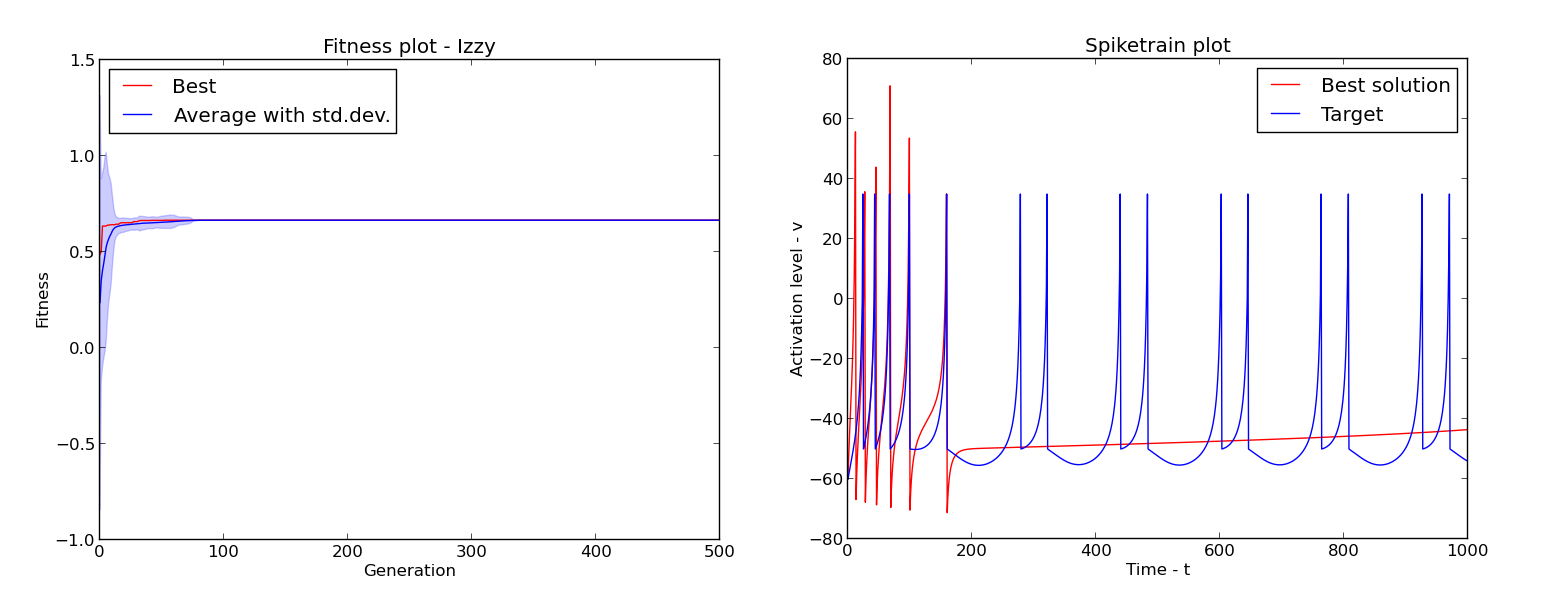
\includegraphics[width=1.2\textwidth]{img/case2_wave}}
% [0.001, 0.1267632624468753, -80.0, 8.831074063189003, 0.06096717156823159]
% 0.665574684289
Best solution: 
a: 0.001 
b: 0.1267 
c: -80 
d: 8.831 
k: 0.0609 \\
Fitness: 0.6656
\paragraph{}This one starts out good, and then completely flatlines after about t=180. Looking at the bottoms of the spikes we see that these have a different shape from the ones in the target. This suggests that we may be stuck in the wrong part of the solution space.

\subsubsection{Spike Time Distance Metric}
\centerline{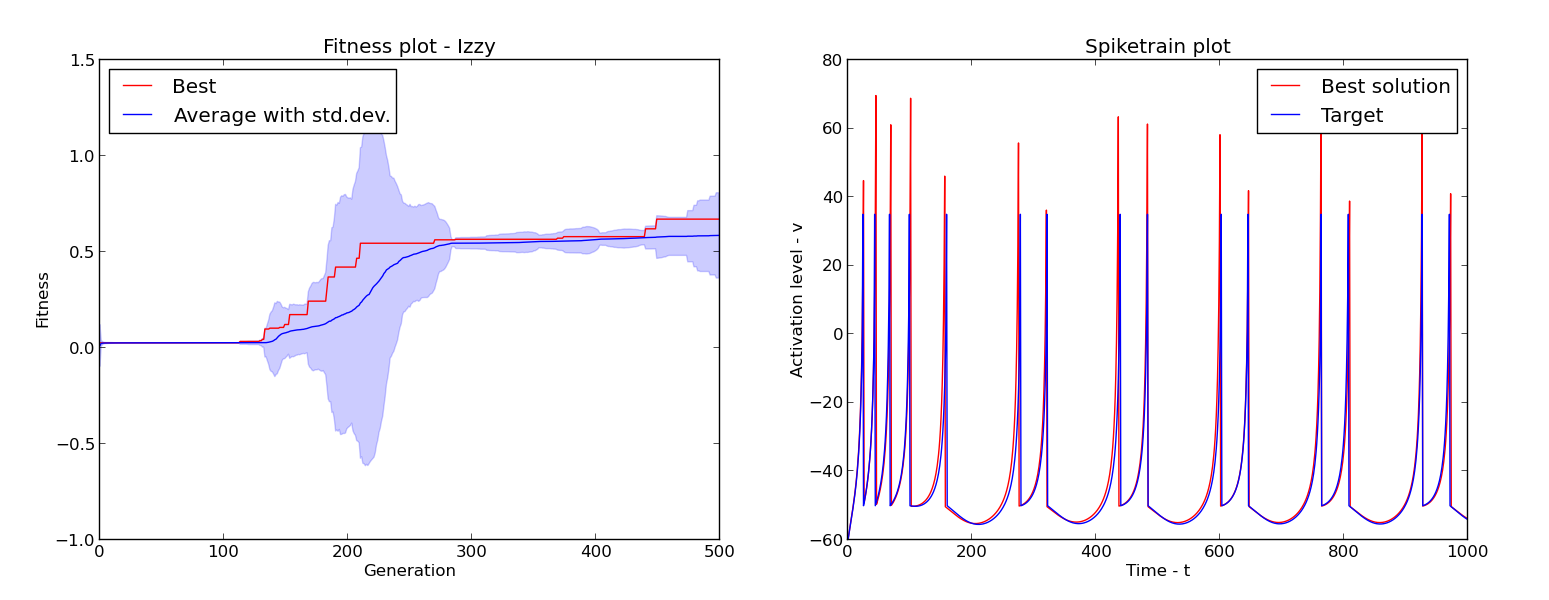
\includegraphics[width=1.2\textwidth]{img/case2_time}}
% [0.0245620948715795, 0.18322939561856222, -50.14289487904963, 3.909108243074065, 0.0451019688547179]
% 0.671186909794
Best solution: 
a: 0.02456 
b: 0.1832 
c: -50.14 
d: 3.909 
k: 0.04510 \\
Fitness: 0.6712
\paragraph{}Very good solution, and still improving near the end of the run.

\subsubsection{Spike Interval Distance Metric}
\centerline{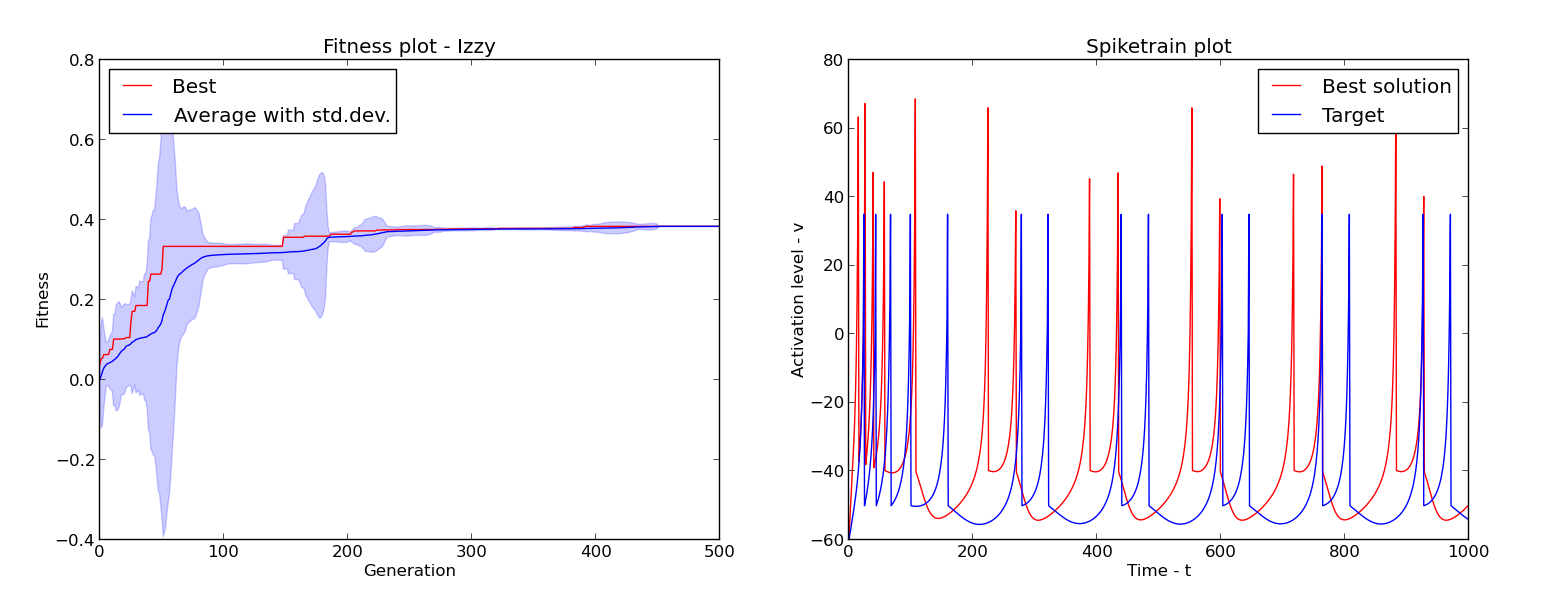
\includegraphics[width=1.2\textwidth]{img/case2_int}}
% [0.03495487629166548, 0.029564089561062414, -39.64871691232427, 10.0, 0.05348620808632682]
% 0.384088378211
Best solution: 
a: 0.03495 
b: 0.02956 
c: -39.65 
d: 10 
k: 0.05349 \\
Fitness: 0.3841
\paragraph{}Once again the waveform is moved to one side, but (according to the eyeball test) it seems that this is a much smaller problem here.

\subsection{Training Data Set 3}
\subsubsection{Waveform Distance Metric}
\centerline{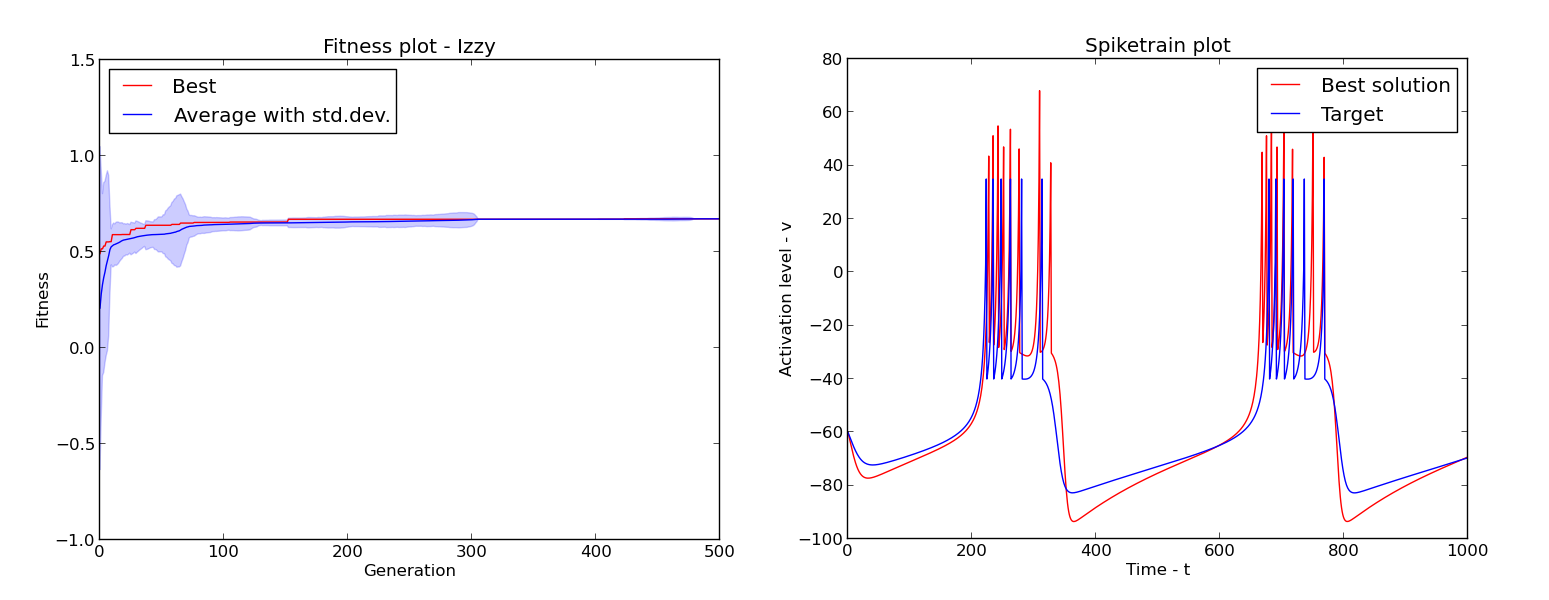
\includegraphics[width=1.2\textwidth]{img/case3_wave}}
% [0.09712347773406639, 0.21478669688766144, -30.0, 9.589098812462376, 0.03890530918056051]
% 0.672842946564
Best solution: 
a: 0.09712 
b: 0.2148 
c: -30 
d: 9.589 
k: 0.03891 \\
Fitness: 0.6728
\paragraph{}The number of spikes is of course all wrong, but the general shape of the solution is definitely there. The non-spiking portion of the target has a very characteristic shape here, which may be part of the reason why waveform works so well here.

\subsubsection{Spike Time Distance Metric}
\centerline{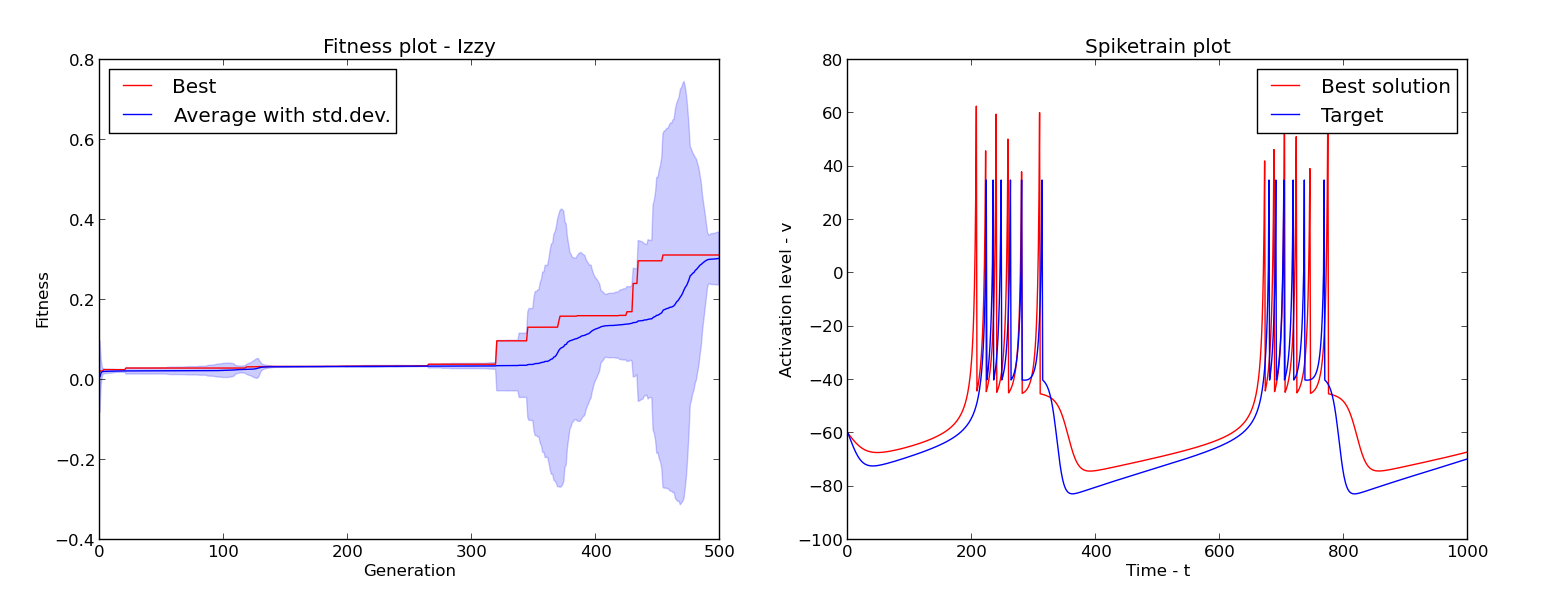
\includegraphics[width=1.2\textwidth]{img/case3_time}}
% [0.03341580902646693, 0.17122258701172716, -45.10862081998512, 2.626080038566368, 0.040830378028918035]
% 0.312493835043
Best solution: 
a: 0.0334 
b: 0.1712 
c: -45.11 
d: 2.6261 
k: 0.04083 \\
Fitness: 0.3125
\paragraph{}We have the right number of spikes, and the general shape down. The fitness plot shows us we're nowhere near done, so this one has potential.

\subsubsection{Spike Interval Distance Metric}
\centerline{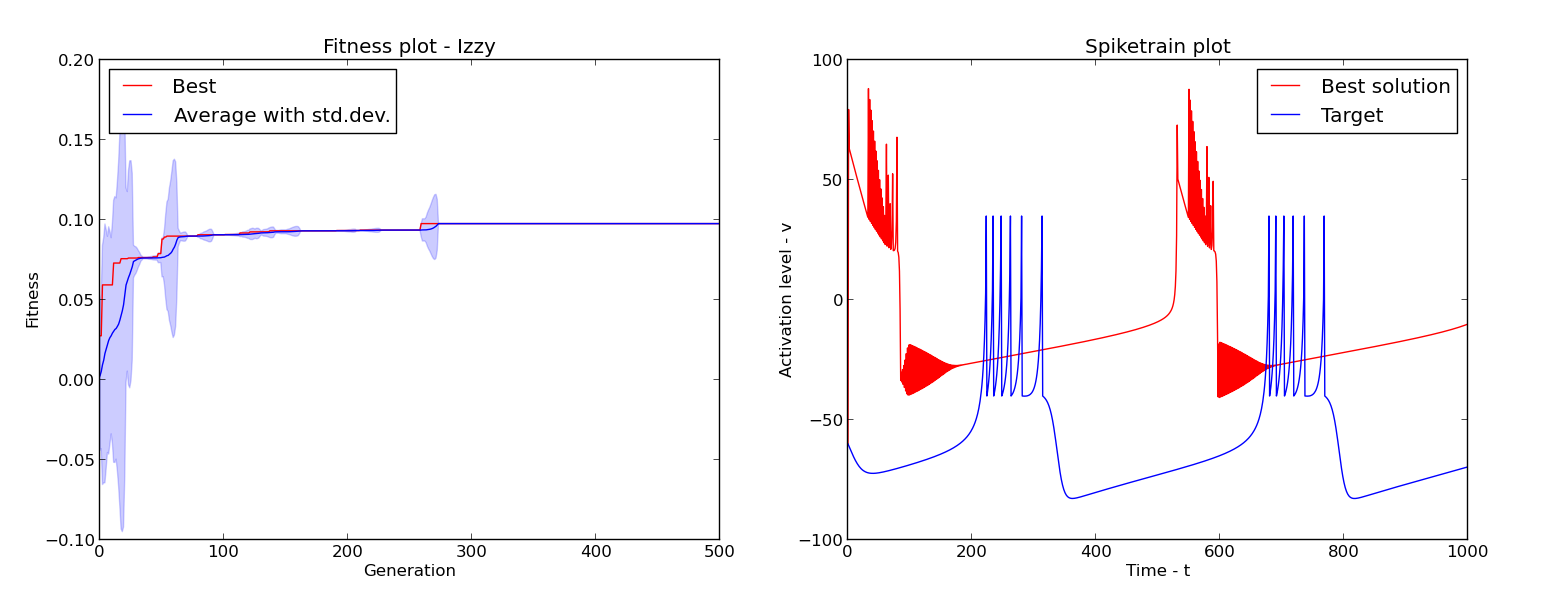
\includegraphics[width=1.2\textwidth]{img/case3_int}}
% [0.026641980766987462, 0.28375896316160454, -55.57964072740265, 9.989149246616881, 0.42883078500127547]
% 0.0977488912107
``Best'' solution: 
a: 0.02664 
b: 0.2838 
c: -55.58 
d: 9.989 
k: 0.4288 \\
Fitness: 0.09774
\paragraph{}No amount of tweaking parameters got us a good solution here. Notice the blocks of solid color, which we can only assume are periods of one spike every other tick. The triangular shapes near the top will probably be interpreted as a single spike, due to the window size being 5. Verdict: Not even close. If we were evolving movies, this one would be \textit{Plan 9 from Solution Space}.

\subsection{Training Data Set 4}
\subsubsection{Waveform Distance Metric}
\centerline{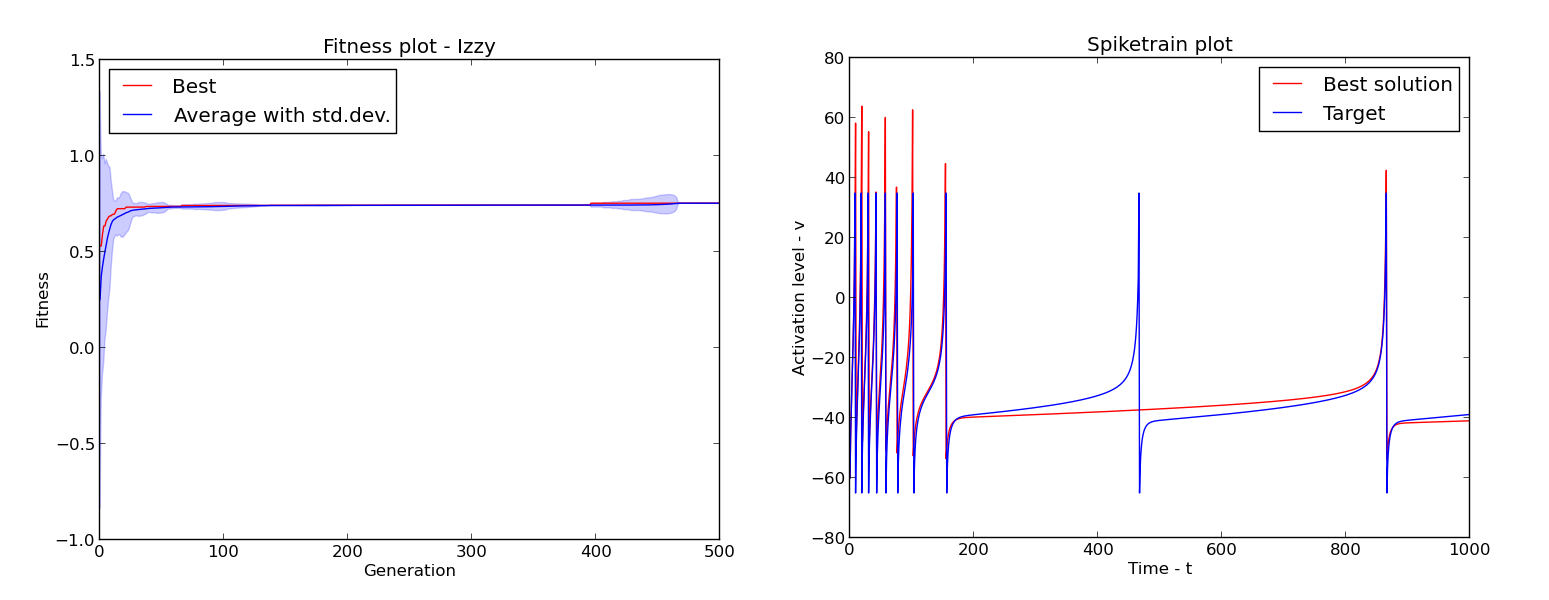
\includegraphics[width=1.2\textwidth]{img/case4_wave}}
% [0.0013246729594224467, 0.028040355581305416, -59.11141487558183, 9.80951824442399, 0.07970806034563727]
%0.754402550013
Best solution: 
a: 0.00132 
b: 0.02804 
c: -59.11 
d: 9.810 
k: 0.07971 \\
Fitness: 0.7544
\paragraph{}Not all that bad, but again the middle spike is missing.

\subsubsection{Spike Time Distance Metric}
\centerline{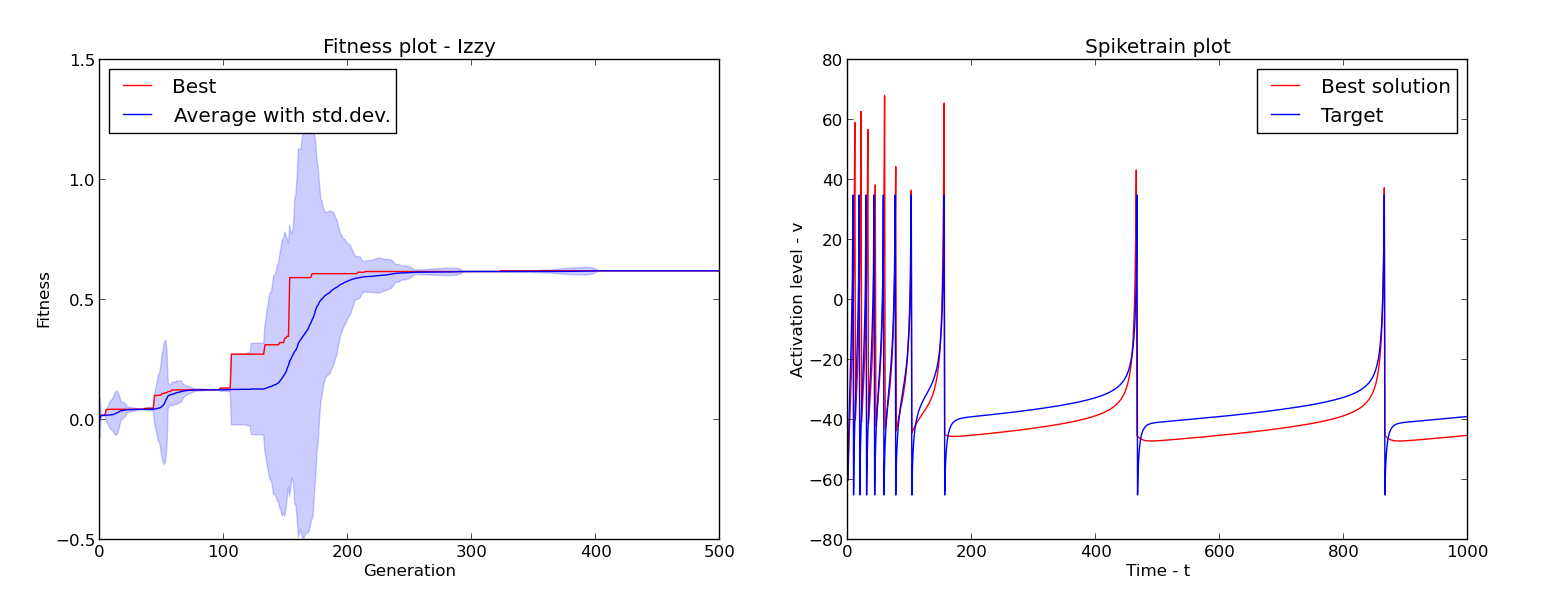
\includegraphics[width=1.2\textwidth]{img/case4_time}}
% [0.00309652283270591, 0.10578502590502979, -44.918896372218924, 7.576631337601864, 0.06568983494734311]
% 0.621783725349
Best solution: 
a: 0.0031 
b: 0.1058 
c: -44.92 
d: 7.577 
k: 0.06569 \\
Fitness: 0.6218
\paragraph{}The spikes line up almost perfectly, but the bottoms have the wrong shape. We are unsure if this is relevant for further use in artificial neural networks.

\subsubsection{Spike Interval Distance Metric}
\centerline{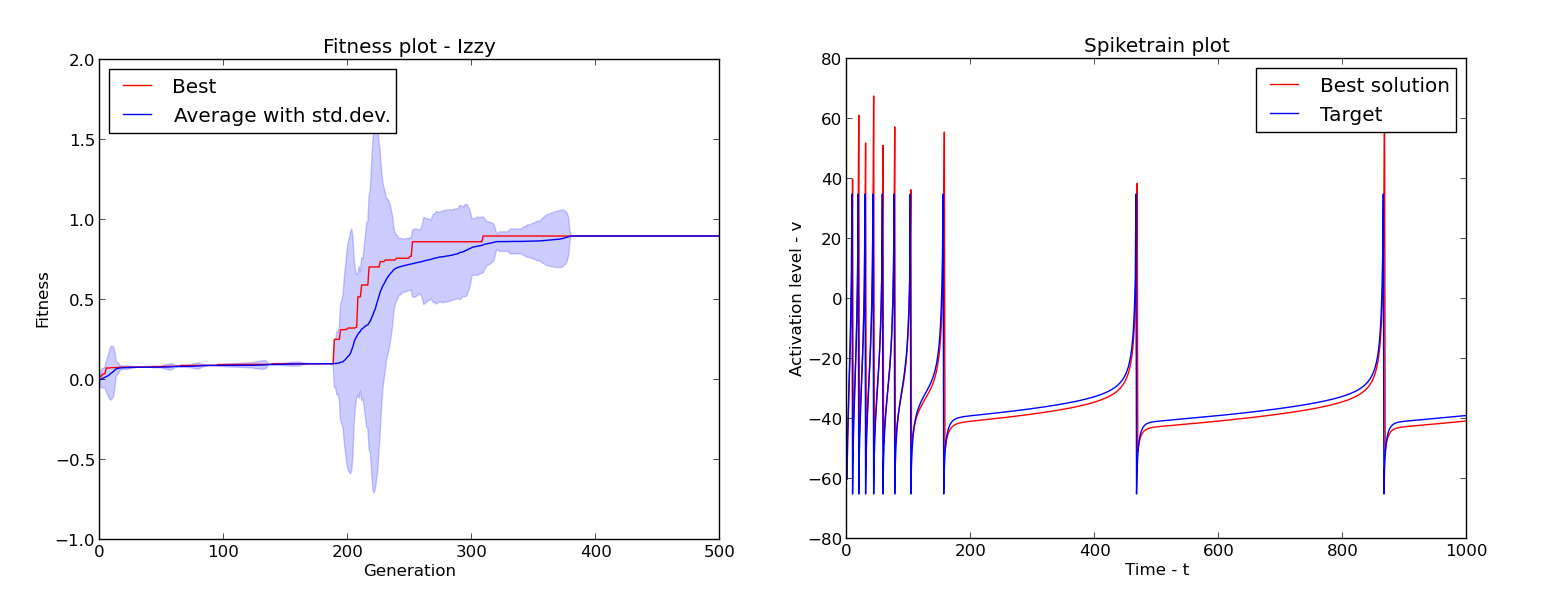
\includegraphics[width=1.2\textwidth]{img/case4_int}}
% [0.003041631477576146, 0.1951214140943149, -53.23426920555409, 9.326047947510688, 0.07540571509624523]
% 0.9
Best solution: 
a: 0.00304 
b: 0.1951 
c: -53.23 
d: 9.326 
k: 0.07541 \\
Fitness: 0.9
\paragraph{}Almost perfect. Once, while testing the code, this combination of SDM and test data attained a fitness of 1.0 in just 14 generations, so we can conclude that this SDM is very well suited for evolving this type of spiketrain.

\section{Discussion}
\subsection{Genotype--phenotype Mapping}
\paragraph{}The mapping is data-oriented, since the values in the genotype are used as input data for a fixed algorithm. The developmental effort is quite high, since computing a spiketrain from the parameter values requires doing a lengthy numerical computation. There is, however, high correlation between the genotype and phenotype, since a small change in the genotype doesn't change the phenotype much. This would be very different if we'd used e.g. a bit vector, where a single bit flipping can cause a huge change in numerical value, and hence the phenotype.

\subsection{Practical Implications}
\paragraph{}Bursting is a phenomenon that is observed in certain naturally occuring neurons. Since computational neuroscience tries to mimic natural neural networks, it is useful to have a computational model for this type of behavior. If one knows that a naturally occuring neuron bursts according to a specific pattern, one could use this tool to evolve the parameters to accurately model it, and use these in an ANN simulation.

\subsection{Other Problem Domains}
Any system where you have a time-varying response based on some external output could potentially be a candidate here. The stock market is one example. One could create a model of the stock market as a function of some collection of external factors, with unknown weights for each factor, and then use this evolutionary algorithm to find these weights. One would then (possibly) have a good model that could be used to predict future stock market trends. The challenge would of course be coming up with the function.

\end{document}
